\section{Introducción}

El trazado de rayos (o \emph{ray-tracing}, como es conocido en inglés) es una técnica usada para la generación de imágenes simuladas que representan objetos posicionados en un espacio tridimensional. Este algoritmo simula el paso de un rayo de luz a través de los pixeles en la imagen a generar, entonces calculando el color que tendría ese píxel si fuera visto a través de una cámara convencional. Este algoritmo tiene alto grado de realismo, si bien es a expensas de un costo computacional alto, lo que no lo hace conveniente para procesos que requieran una respuesta en tiempo real, tales como videojuegos, simuladores, etc. En cambio, este tipo de algoritmos es muy usado en otras aplicaciones donde el tiempo de respuesta no es un inconveniente, tales como la animación de peliculas (algunos ejemplos son \emph{Toy Story} o \emph{Finding Nemo} de Pixar Inc.), o la generación de representaciones realistas de objetos o edificios a construir a partir de planos digitales.
En nuestro algoritmo, implementamos dos primitivas elementales: la esfera o el triángulo. A través de estas, se pueden aproximar prácticamente cualquier objeto que se quiera representar, sin la necesidad de crear una subrutina para cada una de ellos. En la figura 1 se pueden apreciar representaciones de una esfera y un tetraedro generadas por el algoritmo de trazado de rayos. La primera está generada a partir de su primitiva, y el segundo está generado a partir de 4 triángulos, uno por cada cara.\\

\begin{figure}[H]
	\begin{center}
		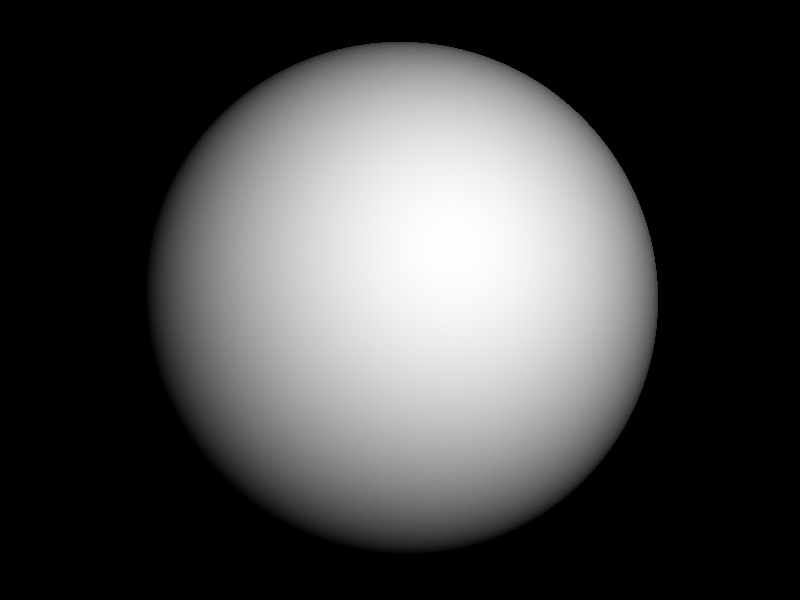
\includegraphics[scale=0.2]{sphere1.jpg}
		\hspace{1.5cm}
		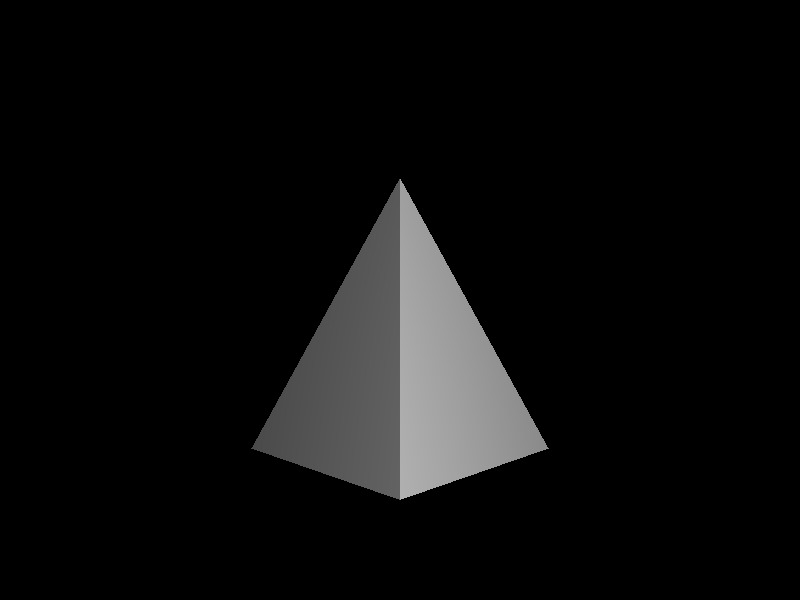
\includegraphics[scale=0.2]{tetrahedron1.jpg}
	\end{center}		
	\caption{Esfera y tetraedro generados por el algoritmo de trazado de rayos}
	\label{fig1}
\end{figure}

Vamos a dividir el trabajo en cuatro partes. En la primera, proveeremos una explicación de los temas de matemática y física que aplicamos para la construcción del algoritmo. En la segunda parte,  explicaremos el algoritmo propiamente dicho, con su correspondiente cálculo de complejidad. En la tercera parte, explicaremos como se llevo a cabo la vectorización de dicho algoritmo, explicando las optimizaciones realizadas. Finalmente, experimentaremos con algunos casos de prueba para medir las mejoras en la práctica que nos da la vectorización y realizaremos el análisis pertinente.